\documentclass{article}
\usepackage{graphicx}
\usepackage{booktabs}
\usepackage{bm}
\usepackage[margin=1in]{geometry}

\title{Analysis of Metrics for Proactive Intervention}
\author{}
\date{}

\begin{document}
\maketitle

\section{Introduction}
Evaluating proactive robotic interventions requires metrics that capture not only the correctness of an action but also its necessity and temporal alignment. Standard event-level metrics such as F1 score or mean Intersection over Union (mIoU) frequently fail to penalize specific types of prediction errors, as demonstrated by our synthetic adversaries analysis. We propose the A-Score to address these gaps.

\section{Methodology}
We simulate diverse failure modes using synthetic prediction tracks generated from ground truth (GT) interventions. The behaviors include a "Spammer" that fires rapidly, a "One-shot blanket" prediction covering the entire task window, and "Right-time-wrong-action". We score these adversaries using base event-level baselines (F1, mIoU, mAcc) alongside the component scores of A-Score: $A_{time}$, $A_{act}$, and $A_{nec}$.

\section{Results}
Table~\ref{tab:results} summarizes the performance of various synthetic adversaries. Noticeably, standard metrics provide incomplete pictures. For example, a predictive model that triggers right before or right after the ideal window ("Near-miss timing") might score highly on F1 if its bounding box partially overlaps the GT event appropriately, but it falls short representing an actual precise supportive action. Notice how \textit{Spammer} achieves non-trivial Event-F1 (0.40) despite being fundamentally useless for robotic assistance, whereas its A-Score properly collapses to 0.15 precisely due to $A_{act}$ and $A_{time}$ penalties. Conversely, \textit{Right-time-wrong-action} achieves perfect Event-F1 on boundary detection but fails entirely on matching the correct skill.

Figure~\ref{fig:timeline} visually portrays these adversarial prediction timelines against the GT track. The visualization clearly shows the qualitative differences between predicting broadly over the entire timeline vs precise temporal coverage.

\begin{table}[h]
\centering
% Generated by scripts/eval/ascore_adversaries.py
\begin{tabular}{lrrrrrrrr}
\toprule
\textbf{Adversary} & \textbf{F1} & \textbf{mIoU} & \textbf{mAcc} & $\bm{P_{agree}}$ & $\bm{A_{time}}$ & $\bm{A_{act}}$ & $\bm{A_{nec}}$ & $\bm{A_{score}}$ \\
\midrule
Oracle & 1.00 & 1.00 & 1.00 & 1.00 & 1.00 & 1.00 & 1.00 & 1.00 \\
Silent & 0.00 & 0.00 & 0.00 & 0.35 & 0.00 & 0.00 & 1.00 & 0.33 \\
Spammer & 0.40 & 0.00 & 0.20 & 0.19 & 0.00 & 0.20 & 0.25 & 0.15 \\
One-shot blanket & 0.33 & 0.15 & 1.00 & 0.15 & 0.03 & 0.20 & 1.00 & 0.41 \\
Right-time-wrong-action & 1.00 & 1.00 & 0.00 & 0.35 & 1.00 & 0.00 & 1.00 & 0.67 \\
Near-miss timing & 0.80 & 0.38 & 0.00 & 0.23 & 0.31 & 0.00 & 0.95 & 0.42 \\
Far-shifted & 0.75 & 0.36 & 0.00 & 0.20 & 0.21 & 0.00 & 1.00 & 0.40 \\
Premature firer & 1.00 & 0.00 & 1.00 & 0.15 & 0.00 & 1.00 & 1.00 & 0.67 \\
Over-extender & 1.00 & 0.34 & 1.00 & 0.75 & 0.34 & 1.00 & 1.00 & 0.78 \\
Half-coverage perfect & 0.75 & 1.00 & 1.00 & 0.75 & 0.60 & 0.60 & 1.00 & 0.73 \\
\bottomrule
\end{tabular}
% match tolerance = 15.0s, weights = (0.333, 0.333, 0.333)
\caption{Quantitative evaluation of synthetic adversaries against ground truth interventions across different evaluation metrics.}
\label{tab:results}
\end{table}

\begin{figure}[h]
\centering
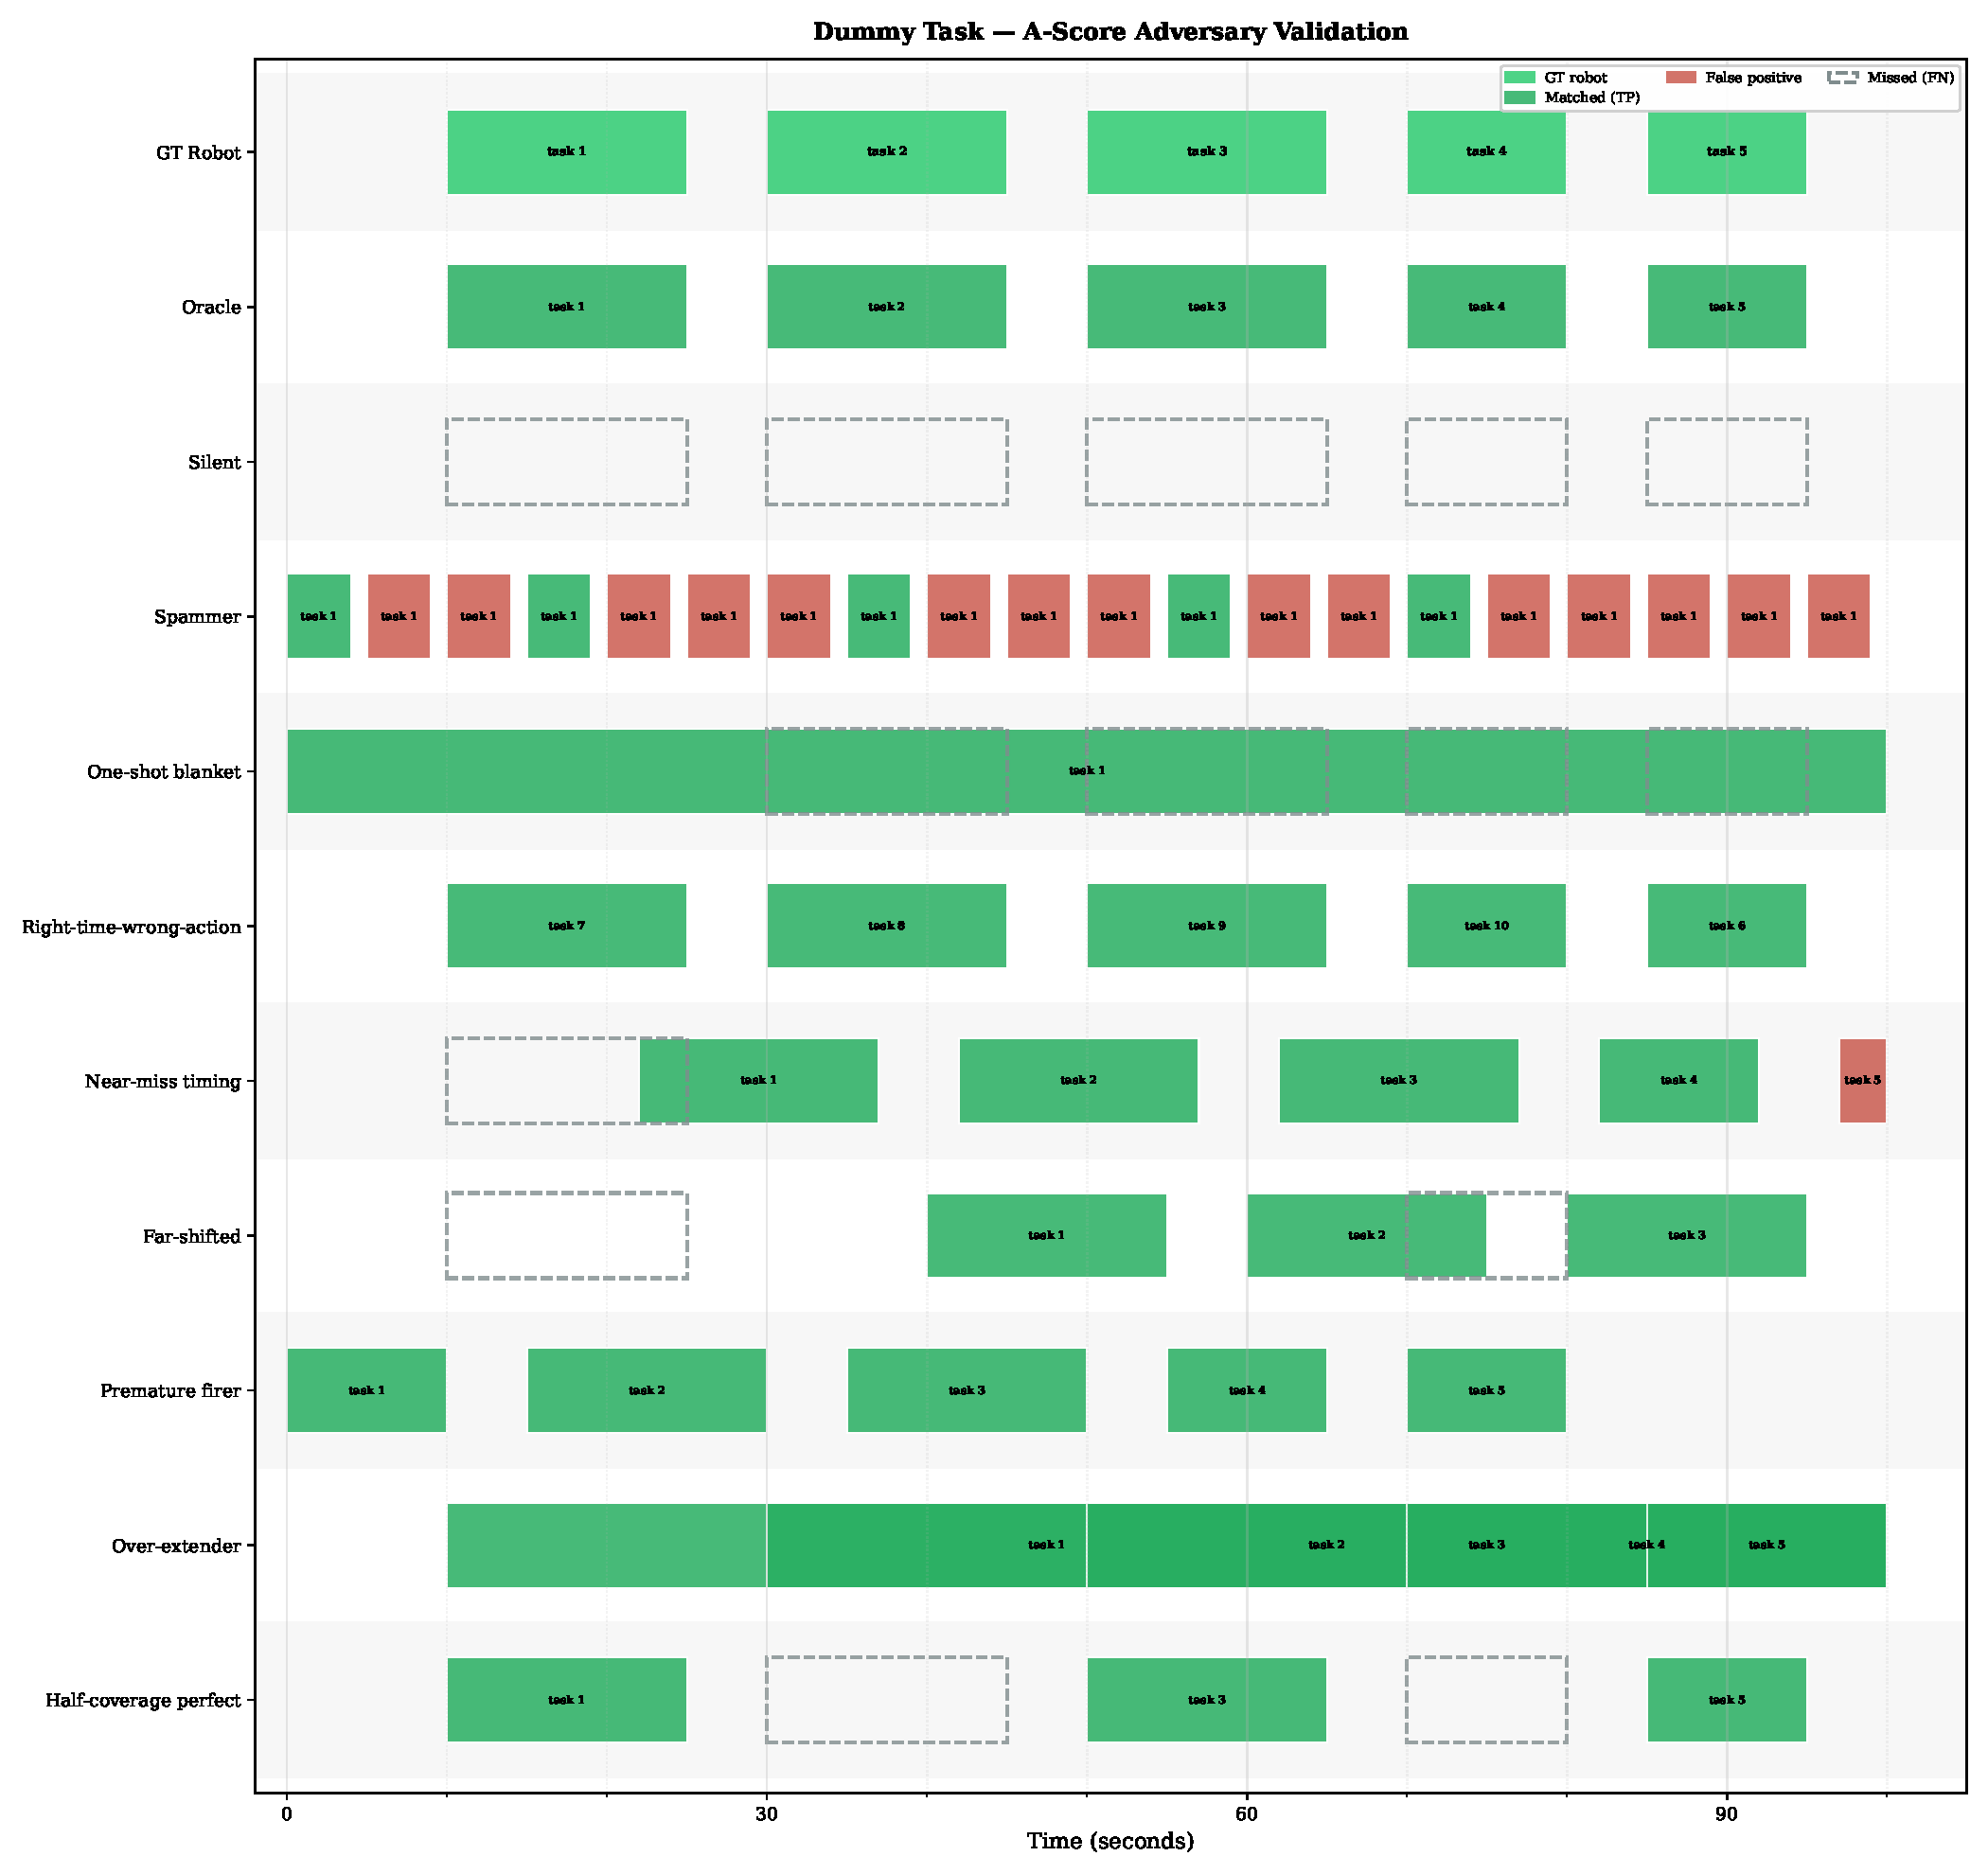
\includegraphics[width=\textwidth]{../../../figures/generated/fig_ascore_adversaries_dummy.pdf}
\caption{Visualized timelines of adversary behaviors compared to Ground Truth.}
\label{fig:timeline}
\end{figure}

\end{document}
